%!TEX program =pdflatex
\documentclass{beamer}
\usetheme{CambridgeUS}
%%define new comand
\def\argmin{\mathop{\rm arg~min}\limits}
\def\argmin{\mathop{\rm arg~min}\limits}
\newcommand{\bdelta}{\boldsymbol{\delta}}
\newcommand{\bbeta}{\boldsymbol{\beta}}
\newcommand{\bSigma}{\boldsymbol{\Sigma}}
\newcommand{\brho}{\displaystyle{\large{\boldsymbol{\rho}}}}
\newcommand{\bgamma}{\boldsymbol{\gamma}}
\newcommand{\bfeta}{\boldsymbol{\eta}}
\newcommand{\bPsi}{\boldsymbol{\Psi}}
\newcommand{\bmu}{\boldsymbol{\mu}}
\newcommand{\bvartheta}{\boldsymbol{\vartheta}}
\newcommand{\bzero}{\mathbf{0}}
\newcommand{\bone}{\mathbf{1}}
\newcommand{\bA}{\mathbf{A}}
\newcommand{\ba}{\mathbf{a}}
\newcommand{\bB}{\mathbf{B}}
\newcommand{\bb}{\mathbf{b}}
\newcommand{\bD}{\mathbf{D}}
\newcommand{\bU}{\mathbf{U}}
\newcommand{\bu}{\mathbf{u}}
\newcommand{\bV}{\mathbf{V}}
\newcommand{\bW}{\mathbf{W}}
\newcommand{\bw}{\mathbf{w}}
\newcommand{\bX}{\mathbf{X}}
\newcommand{\bx}{\mathbf{x}}
\newcommand{\bY}{\mathbf{Y}}
\newcommand{\by}{\mathbf{y}}
\newcommand{\bZ}{\mathbf{Z}}
\newcommand{\bz}{\mathbf{z}}
\newcommand{\suit}[1]{\left(#1\right)}
\newcommand{\abs}[1]{\left\vert#1\right\vert}
\newcommand{\set}[1]{\left\{#1\right\}}
\newcommand{\msuit}[1]{\left[ #1 \right]}
\newtheorem{prop}{Proposition}[section]
\author{Z. Zhao, Z. Zhang, R. Chen}
\title{Modeling Maxima with autoregressive conditional Fr\'echet model}
\begin{document}
\begin{frame}
\titlepage
\begin{center}
    Published on Journal of Econometrics (2018)
    \bigskip

    Presented by Liujun Chen
    \bigskip
    \bigskip
\end{center}
\end{frame}
\AtBeginSection[]
{
\begin{frame}
\frametitle{Table of Contents}
\tableofcontents[currentsection]
\end{frame}
}


\section{Introduction}

\begin{frame}
    \frametitle{Introduction}
    Maximum
    observations, as the representation of extreme behavior, are of particular interest.
    \bigskip
\begin{itemize}
    \item mutual fund managers: the potential maximum daily loss across all stocks in their managed portfolio
    \bigskip
    \item high-frequency traders: the level of potential
    intra-day maximum loss 
\end{itemize}
    

\end{frame}

\begin{frame}
    \frametitle{Introduction}
    Most applications of EVT focus on modeling extreme events in time series with a
    static approach under equilibrium distribution.
    
    \bigskip
    \begin{itemize}
        \item  The behavior of the underlying time series may change through
        time. 
        \bigskip
        \item  Financial time series tends to exhibit structural changes and time-varying dynamics such as volatility clustering.
    \end{itemize}
\end{frame}


\begin{frame}
    \frametitle{Introduction}
    Model time series of maxima $\set{Q_t}$, where $\set{Q_t}$ is a univariate time series
    of maxima based on a set of underlying financial time series $\set{X_{it}}_{i=1}^p$. There are mainly two types of $Q_t$.
    \bigskip

    \begin{itemize}
        \item time series of cross-sectional maxima e.g. modeling the maximum daily loss across a group of stocks in a portfolio
        \bigskip
        \item the time series of intra-period maxima e.g. intra-day maxima of high-frequency
        trading losses that occur on the same day.
    \end{itemize}

\end{frame}


\section{Autoregressive conditional Fr\'echet Model}

\begin{frame}
    \frametitle{Dynamic Model}
    \begin{itemize}
        \item     A dynamic GEV framework: a conditional evolution scheme is designed for the parameters $(\mu_t,\sigma_t,\xi_t)$ of GEV, so that time dependency of $\set{Q_t}$ can be captured.
        \bigskip
        \item Due to the heavy-tailedness of financial data, $\set{Q_t}$ can marginally can
        be well modeled by Fr\'echet distribution.
        \item  
        $$
Q_t = \mu_t +\sigma_t Y_t^{1/\alpha_t},
        $$
        where $Y_t$ is a sequence of i.i.d. unit Fr\'echet random variables.
    \end{itemize}
\end{frame}


\begin{frame}
    \frametitle{Should $\alpha_t$ be dynamic?}
\begin{itemize}
    \item Ad-hoc moving-window GEV analysis on the cross-sectional maxima of negative daily log-returns of S\&P 100 index
    \item The observation period is from January 1, 2000 to     December 31, 2014 with 3773 trading days.
    \item For each trading day t, we record the maximum daily loss across the 100 stocks
    and denote it by $Q_t$, Hence the time series $\set{Q_t}$ has 3773 observations
    \item For each $500\le t\le 3273$, a GEV model is fitted using $\set{Q_k}_{k=t-499}^{t+500}$.
\end{itemize}
\end{frame}


\begin{frame}
    \frametitle{Moving Window Estimatio of Tail Index $\alpha$}
    \begin{figure}
        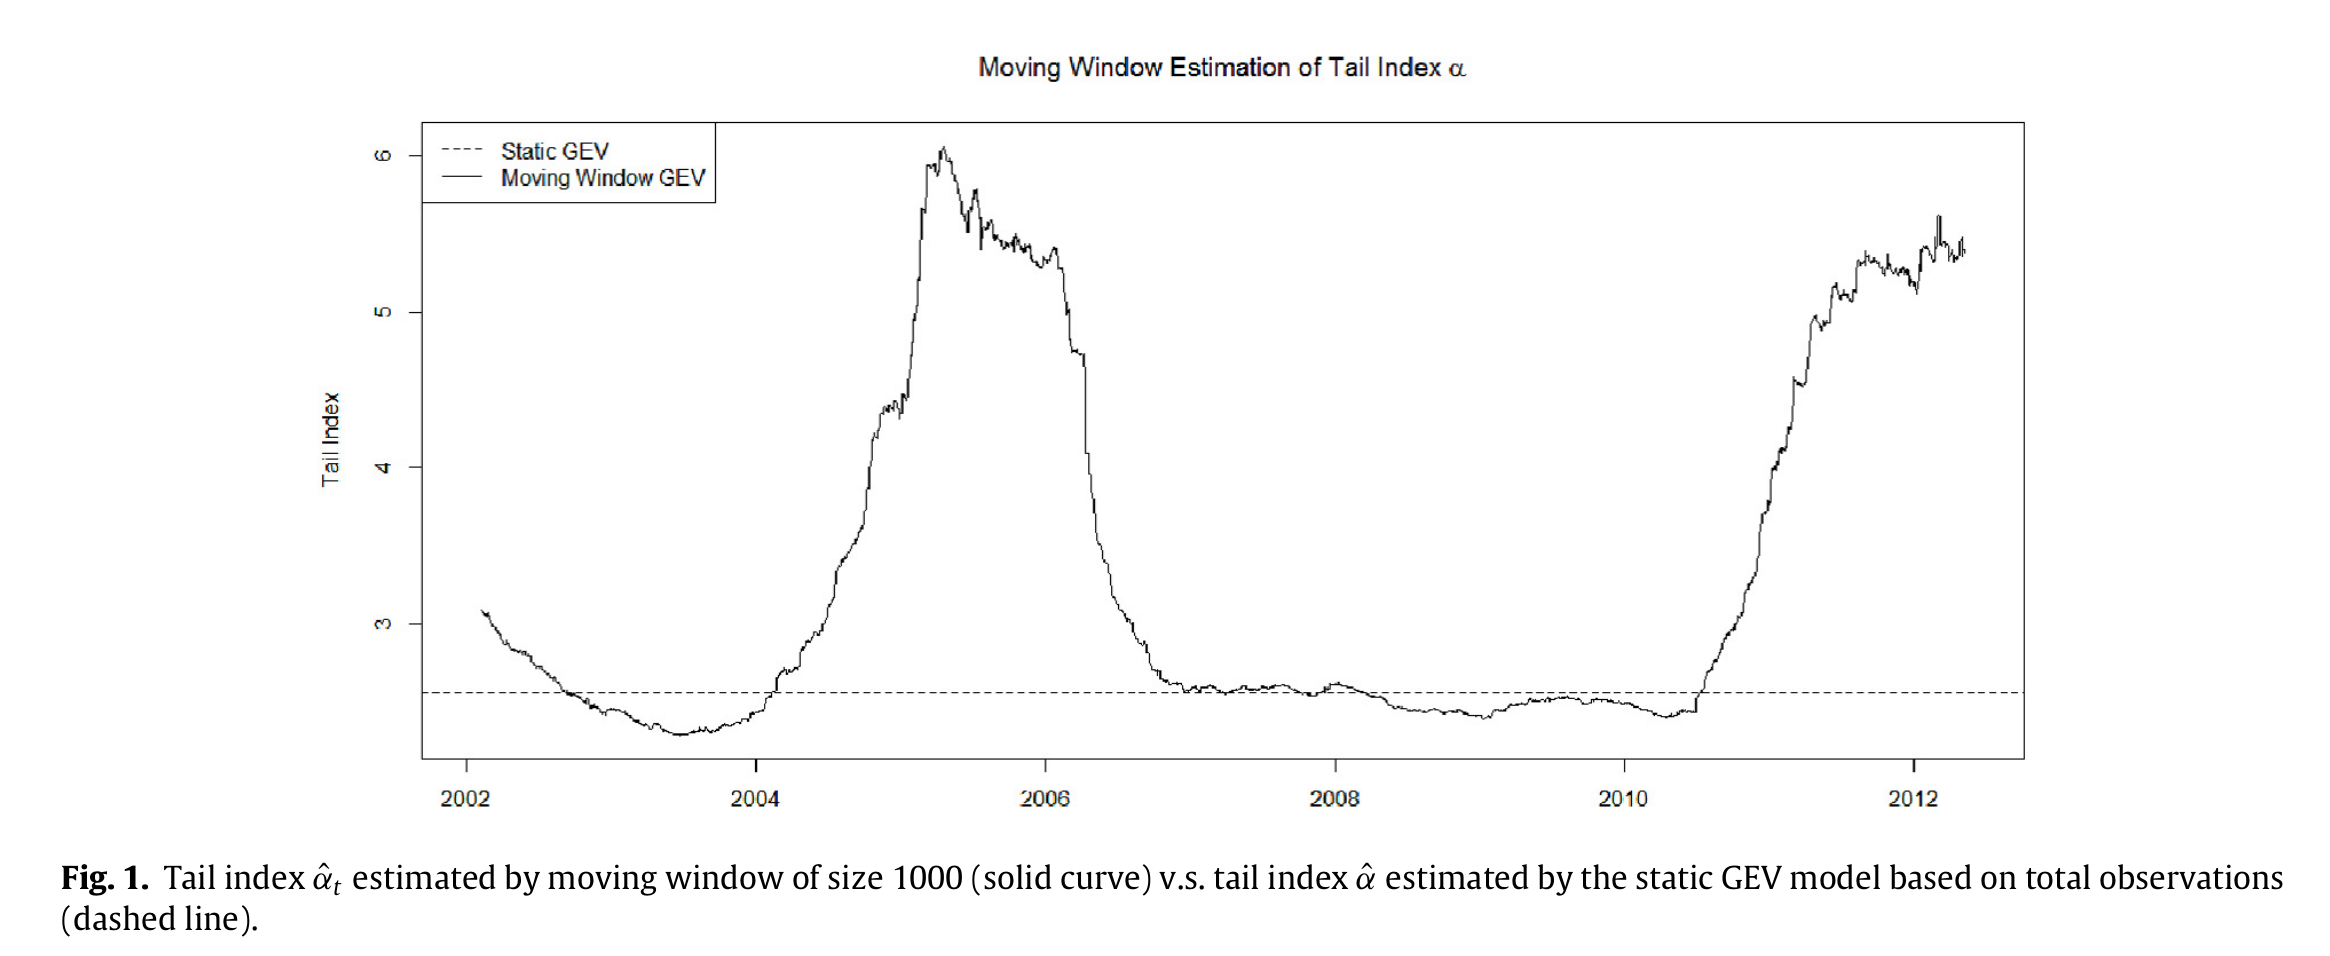
\includegraphics[width=1\textwidth]{fig1.png}   
    \end{figure}
\end{frame}


\begin{frame}
    \frametitle{Model Specification}
    Specifically, the autoregressive conditional Fr\'echet(AcF) model assumes the form  
    $$
\begin{aligned}
 \log \sigma_t & = \beta_0 +\beta_1 \log \sigma_{t-1}+\eta_1(Q_{t-1}) \\
    \log \alpha_t &=\gamma_0+\gamma_1 \log \sigma_{t-1}+\eta_2(Q_{t-1}) ,
\end{aligned}
    $$
    where $\beta_1,\gamma_1\ge 0$. The log
    transform is used to ensure the positivity of the parameters.

    \bigskip

    Assume that $\eta_1$ is a continuous increasing function and $\eta_2$ is a continuous decreasing function of $Q_{t-1}$. Choose $\eta_1,\eta_2$ to be the simple exponential function $a_0\exp\suit{-a_1 x}$.
\end{frame}

\begin{frame}
    \frametitle{Model Specifiction}

    For the rest of the paper, we consider the following model:
  \begin{equation}\tag{*}
\begin{aligned}
    Q_t& = \mu +\sigma_t Y_t^{1/\alpha_t}, \\
    & \\
 \log \sigma_t & = \beta_0 +\beta_1 \log \sigma_{t-1}-\beta_2\exp(-\beta_3 Q_{t-1}), \\
 & \\
    \log \alpha_t &=\gamma_0+\gamma_1 \log \sigma_{t-1}+\gamma_2\exp(-\gamma_3 Q_{t-1}) ,
\end{aligned}
\end{equation}
where $\set{Y_t}$ is a sequence of i.i.d. unit Fr\'echet random variables, $0\le \beta_1 \ne \gamma_1<1$, $\beta_2, \beta_3,\gamma_2,\gamma_3>0$.
\end{frame}


\begin{frame}
    \frametitle{Remark 1}
    \begin{itemize}
        \item AcF can be easily extended to include $q_1$ autoregressive terms of $\log \sigma_t$ and $\log \alpha_t$, and $q_2$ lagged terms of $\eta(Q_t)$, similar to that of GARCH($q_1,q_2$) model.
        \bigskip
        \item Similar theoretical properties can be derived and similar estimation procedures can be used.
        \bigskip
        \item Our empirical experience shows that the extension does not necessarily improve the performance of the model.
    \end{itemize}

    

\end{frame}


\begin{frame}
    \frametitle{Stationarity and ergodicity}
The model can be written as 
$$
\begin{aligned}
 \log \sigma_t & = \beta_0 +\beta_1 \log \sigma_{t-1}-\beta_2\exp(-\beta_3 (\mu+\sigma_{t-1}Y_{t-1}^{1/\alpha_{t-1}})), \\
 & \\
    \log \alpha_t &=\gamma_0+\gamma_1 \log \sigma_{t-1}+\gamma_2\exp(-\gamma_3  (\mu+\sigma_{t-1}Y_{t-1}^{1/\alpha_{t-1}})) ,
\end{aligned}
    $$
    Hence, $\set{\sigma_t,\alpha_t}$ form a homogeneous Markov chain in $\mathbb{R}^2$.
    
\begin{theorem}[1]
    For an AcF with $\beta_2,\beta_3,\gamma_2,\gamma_3>0$, $\beta_0,\gamma_0,\mu\in \mathbb{R}$ and $0\le \beta_1\ne \gamma_1<1$, the latent process $\set{\sigma_t,\alpha_t}$ is stationary and geometrically ergodic.
\end{theorem}
\end{frame}



\begin{frame}
    \frametitle{AcF under a factor model setting}
    We illustrate that the limiting form of maxima $Q_t$ under a general factor model framework leads to an AcF model.
\begin{itemize}
    \item Assume $\set{X_{it}}_{i=1}^p$ follow a general factor model,
    $$
    X_{it} = f_i(Z_{1t},\dots,Z_{dt})+\sigma_{it}\varepsilon_{it},
    $$ 
    
    \item  $\set{X_{it}}_{i=1}^p$ are observed time series at time $t$, $\set{Z_{1n},\dots,Z_{dn}}$ consist of observed and unobserved factors, $\set{\varepsilon_{it}}_{i=1}^p$ are i.i.d. random noises that are independent with the factors $\set{Z_{id}}_{i=1}^d$.
    \item Assume that $\set{\varepsilon_{it}}_{i=1}^p$ are in the domain of attraction of the Fr\'echet distribution. 
\end{itemize}
    

\end{frame}

\begin{frame}
    \frametitle{Other Assumptions for the factor model}
\begin{itemize}
    \item $\sup_{1\le p<\infty}\sup_{1\le i\le p}f_i(Z_{1t},\dots,Z_{dt})<\infty \ \text{a.s.}$
    \bigskip
    \item $\lim_{p\to \infty} \sum_{i=1}^p \sigma_{it}^{\alpha_t}=\infty$
    \bigskip
    \item $\lim_{p\to \infty} \sup_{1\le i\le p}\frac{\sigma_{it}^{\alpha_t}}{\sum_{j=1}^p\sigma_{it}^{\alpha_t}}=0$
\end{itemize}
\end{frame}


\begin{frame}
    \frametitle{Asymptotic conditional distribution of $Q_t$}
    \begin{prop}[1]
    Given $F_{t-1}$, denote $a_{pt} = 0$ and $b_{pt}=(\sum_{j=1}^p \sigma_{it}^{\alpha_t})^{1/\alpha_t}$, we have, as $p\to \infty$,
    $$
\frac{Q_t-a_{pt}}{b_{pt}} \stackrel{d}{\to} \exp(-x^{-\alpha_t}).
    $$
   \end{prop}
    

\end{frame}

\section{Parameter Estimation}


\begin{frame}
    \frametitle{MLE}
    \begin{itemize}
        \item denote all the parameters in the model by $\theta=(\beta_0,\beta_1,\beta_2,\beta_3,\gamma_0,\gamma_1,\gamma_2,\gamma_3,\mu)$
        \bigskip
        \item   denote $\Theta_s=\set{\theta|\beta_0,\gamma_0,\mu\in \mathbb{R}, 0\le \beta_1,\gamma_1<1,\beta_2,\beta_3,\gamma_2,\gamma_3>0}$
        \bigskip
        \item Assume that all allowable parameters are in $\Theta_s$
        \bigskip
        \item Denote the true parameter by $\beta_0=(\beta_0^0,\beta_1^0,\beta_2^0,\beta_3^0,\gamma_0^0,\gamma_1^0,\gamma_2^0,\gamma_3^0,\mu_0)$
    \end{itemize}
\end{frame}


\begin{frame}
    \frametitle{MLE}
    The conditional p.d.f. of $Q_t$ given $(\mu_t,\sigma_t,\alpha_t)$ is 
    $$
f_t(\theta)=f(Q_t|\sigma_t,\alpha_t)=\alpha_t \sigma_t^{\sigma_t}(Q_t-\mu)^{-(\alpha_t+1)} \exp \set{-\sigma_t^{\alpha_t}(Q_t-\mu)^{-\alpha_t}}.
    $$
    Hence, by conditional independence, the log-likelihood function with observations $\set{Q_t}_{t=1}^{n}$ is 
    $$
    \begin{aligned}
L_n(\theta) & =\frac{1}{n}\sum_{t=1}^n \log f_t(\theta)\\
&=\frac{1}{n}\sum_{i=1}^n \log \alpha_t +\sigma_t \log \sigma_t -(\alpha_t+1) \log(Q_t-\mu)-\sigma_t^{\alpha_t}(Q_t-\mu)^{-\alpha_t}
    \end{aligned}
    $$
where $\set{\sigma_t,\alpha_t}$ can be obtained recursively through (*) with an initial value $(\sigma_1,\alpha_1)$.
    

\end{frame}


\begin{frame}
    \frametitle{Initial Value}
    \begin{itemize}
        \item Notice here the true value of $(\sigma_1,\alpha_1)$, denoted as $(\sigma_1^0,\alpha_1^0)$, is an unknown since the state variables $\set{\sigma_t,\alpha_t}$ is a hidden process.
        \medskip
        \item Fortunately, with $0\le \beta_1,\gamma_1<1$, the influence of $(\sigma_1,\alpha_1)$ on future $(\sigma_t,\alpha_t)$ decays exponentially as $t$ increases
        \medskip
        \item Hence its impact on parameter estimation will be minimum with a sufficiently large sample size.
        \medskip
        \item It will be shown that the consistency and asymptotic normality does not depend on the initial value.
    \end{itemize}
\end{frame}

\begin{frame}
    \frametitle{Asymptotic Properties}
    \begin{theorem}[Consistency]
        Assume the parameter space $\Theta$ is a compact set of $\Theta_s$. Suppose the observations $\set{Q_t}_{t=1}^{n}$ are generated
        by a stationary and ergodic AcF with true parameter $\theta_0$ and $\theta_0$ is in the interior of $\Theta$, then there exists a sequence $\theta_n$ of local maximizer of $L_n(\theta)$ such that $\theta_n \stackrel{p}{\to} \theta_0$ and $||\theta_n-\theta_0||\le \tau_n$ where $\tau_n=O_p(n^{-r}), 0<r<1/2$. Hence $\hat{\theta}_n$ is consistent.
    \end{theorem}
\end{frame}

\begin{frame}
    \frametitle{Asymptotic Properties}
    \begin{prop}[Asymptotic Uniqueness]
        Denote $V_n=\set{\theta\in \Theta|\mu\le cQ_{n,1}+(1-c)\mu_0}$ where $Q_{n,1}=\min_{1\le t\le n}Q_t$, under the conditions in the Theorem for consistency, for any fixed $0<c<1$, there exists a sequence of $\hat{\theta}_n=\arg \max_{\theta\in V_n}\tilde{L}(\theta)$ such that, $\hat{\theta}_n\stackrel{P}{\to}\theta_0$, $||\theta_n-\theta_0||\le \tau_n$ where $\tau_n=O_p(n^{-r}), 0<r<1/2$, and P($\hat{\theta}_n$ is the unique global maximizer of $\tilde{L}_n(\theta)$ over $V_n$) $\to 1$. 
    \end{prop}
\end{frame}

\begin{frame}
    \frametitle{Asymptotic Properties}

    \begin{theorem}[Asymptotic Normality]
        Under the conditions in Theorem for consistency, we have that $\sqrt{n}(\hat{\theta}_n-\theta_0)\stackrel{d}{\to} N(0,M_0^{-1})$, where $\hat{\theta}_n$ is that in Theorem of consistency and $M_0$ is the Fisher Information matrix evaluated at $\theta_0$. Further, the sample variance of plug-in estimated score function $\set{\frac{\partial}{\partial \theta}\log f_t(\hat{\theta}_n)}_{t=1}^n$ is a consistent estimator of $M_0$.
    \end{theorem}

\end{frame}


\section{Simulation Study}

\begin{frame}
    \frametitle{Convergence of maxima in factor model}
\begin{itemize}
    \item we conduct numerical experiments to investigate the finite sample behavior of $Q_t$
    \item Specifically, we study the convergence of the marginal distribution of $Q_t$ to its Fr\'echet limit under a one-time period factor model.
    \item To simplify notation, we drop the time index $t$ in this section.
    \end{itemize}
\end{frame}


\begin{frame}
    \frametitle{Convergence of maxima in factor model}
    We simulate data from the following one-factor
    linear model,
    $$
        X_i=\beta_iZ+\sigma_i\varepsilon_i,\quad i=1,\dots,p,
    $$
    \vspace{-2ex}
\begin{itemize}
    \item $Z\sim N(0,1)$ is the latent model,
    \item $\beta_i$ are i.i.d. random coefficients generated from a uniform distribution $U(-2,2)$
    \item $\varepsilon_i$ are i.i.d.    t-distributions with degree of freedom $v$
    \item $\sigma_i$ are i.i.d. random variables generated from a mixture of
    uniform distribution $\frac{1}{2}U(0.5,1.5)+\frac{1}{2}U(0.75,1.25)$ 
 
\end{itemize}
\end{frame}

\begin{frame}
    \frametitle{Finite sample empirical distribution of the maxima Q and its corresponding Fr\'echet limit}
    \begin{center}
        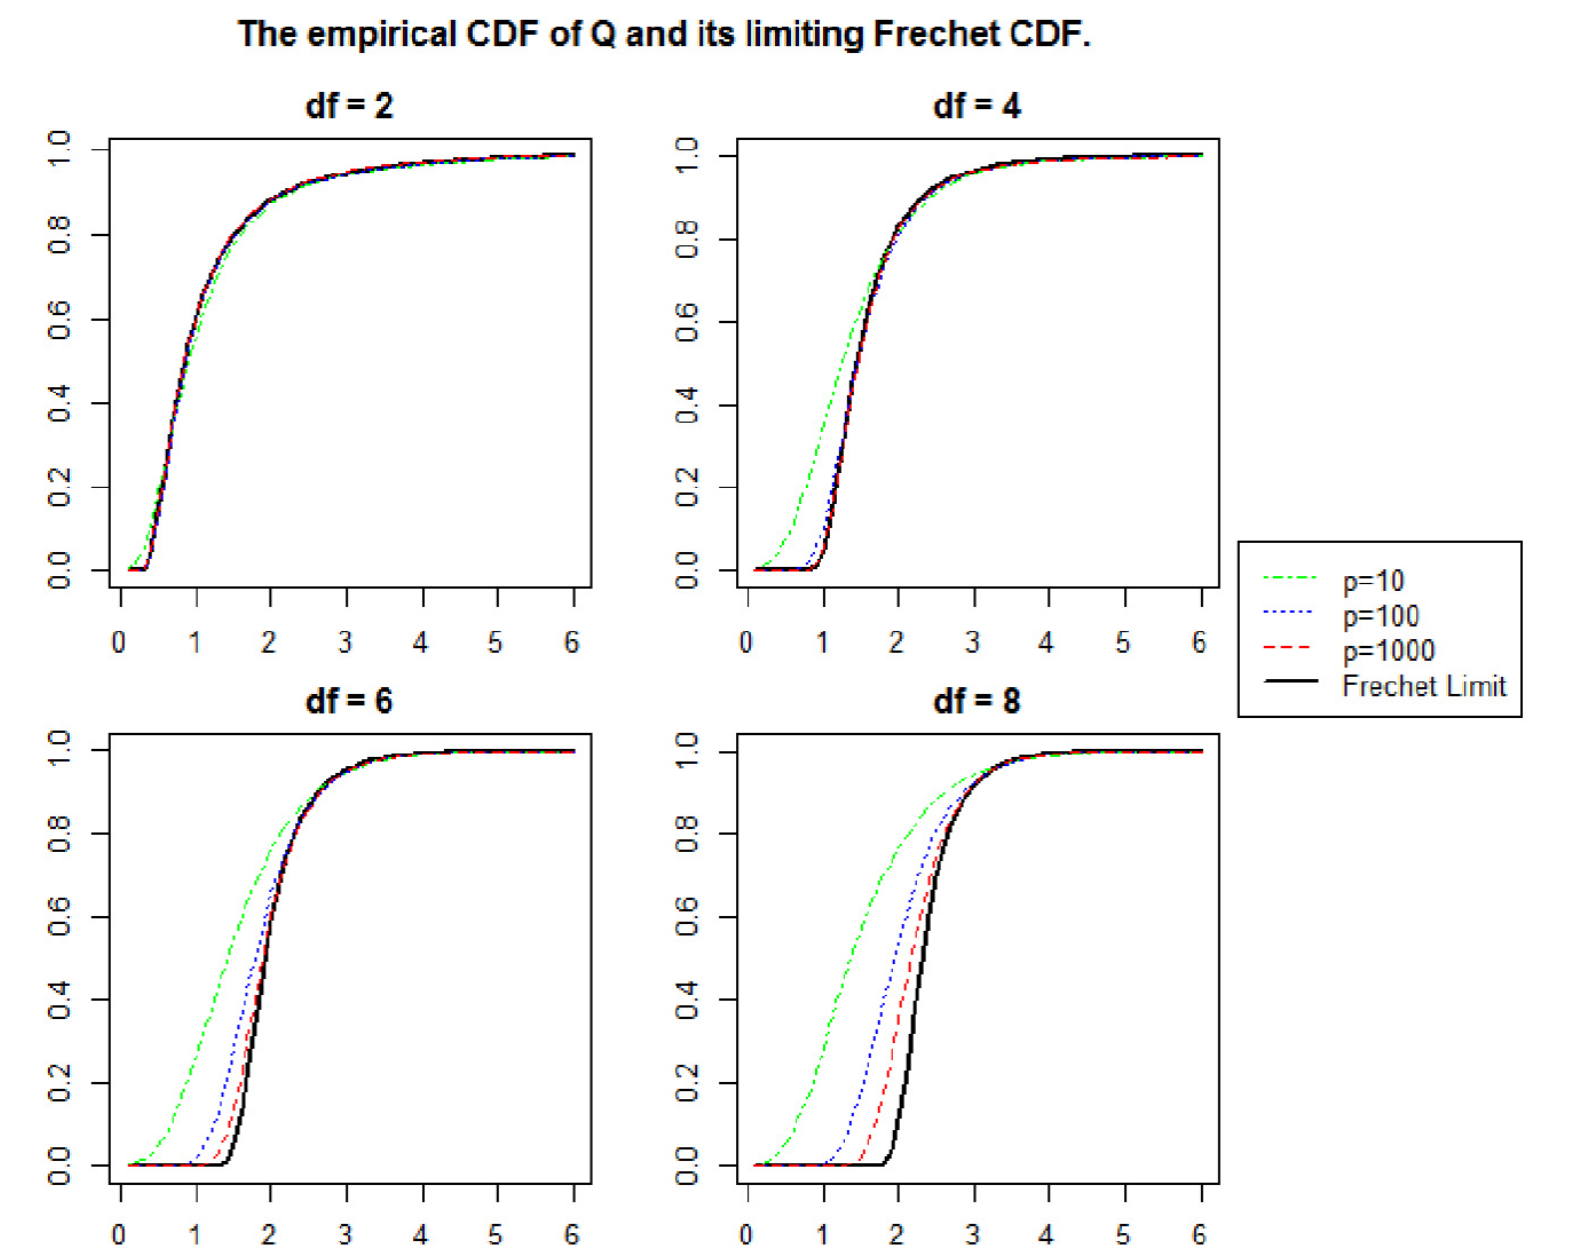
\includegraphics[width=0.7\textwidth]{fig2.png} 
    \end{center}
\end{frame}


\begin{frame}
    \frametitle{AcF estimation for conditional VaR of maxima}
\begin{itemize}
    \item temporal approximation ability of AcF to the maxima $\set{Q_t}$ process from a general factor model
    \bigskip
    \item Model the $\set{Q_t}$ process using AcF and calculate the corresponding $cVaR_t^q$ for $Q_t$ using the fitted AcF.
    \bigskip
    \item $cVaR_t^q$ is defined as the $1-q$ extreme quantile of $Q_t$ given all past information $\mathcal{F}_{t-1}$
\end{itemize}
\end{frame}


\begin{frame}
    \frametitle{Model Setting}
    \begin{itemize}
        \item Simulate $\set{Q_t}$ process from a similar one-factor linear model:
        $$
        X_i=0.09(\beta_iZ_t+\sigma_i\varepsilon_{it}),\quad i=1,\dots,p,
        $$
       
        \item $p=100$
        \bigskip
        \item $v_t=\gamma_0+\gamma_1\log v_{t-1}+\gamma_2\exp(-\gamma_3 Q_{t-1})$ with $(\gamma_0,\gamma_1,\gamma_2,\gamma_3)=(-0.1,0.9,0.3,5)$
        \bigskip
    \end{itemize}
    

\end{frame}

\begin{frame}
    \frametitle{Model Evaluation}
\begin{itemize}
    \item First fit AcF based on the training set $\set{Q_t}_{t=1}^{T_1}$.
    \medskip
    \item Then using fitted AcF, calculate $cVaR_t^q$ for each $Q_t$ on the test set $\set{Q_t}_{t=T_1+1}^{T_1+T_2}$
    \medskip
    \item The true $\set{Q_t}_{t=T_1+1}^{T_1+T_2}$ are then compared with the $\set{cVaR_t^q}_{t=T_1+1}^{T_1+T_2}$ and the number of violations is recorded.
    \medskip
    \item A violation happens when the observed daily maxima $Q_t$ is     larger than the corresponding $cVaR_t^q$ given by AcF.
    \medskip
    \item If AcF approximates the tail behavior of $\set{Q_t}$ process well, the expected proportion of violations in the test set should be close to $q$.
\end{itemize}
    
\end{frame}

\begin{frame}
    \frametitle{Model Evaluation}
    \begin{itemize}
        \item Also, assess the goodness of approximation by calculating the correlation between the true
        process $v_t$ and the estimated process $\hat{\alpha}_t$ by AcF
        \bigskip
        \item $T_1=1000,2000,5000$ $T_2=100$ and $q^0=0.1,0.05,0.01$
        \bigskip
        \item repeat 500 times
        \bigskip
        \item calculate the average violation times $\bar{q}$, mean and the median of the correlation.
    \end{itemize}

    

\end{frame}


\begin{frame}
    \frametitle{Simulation Results}
    \begin{figure}
        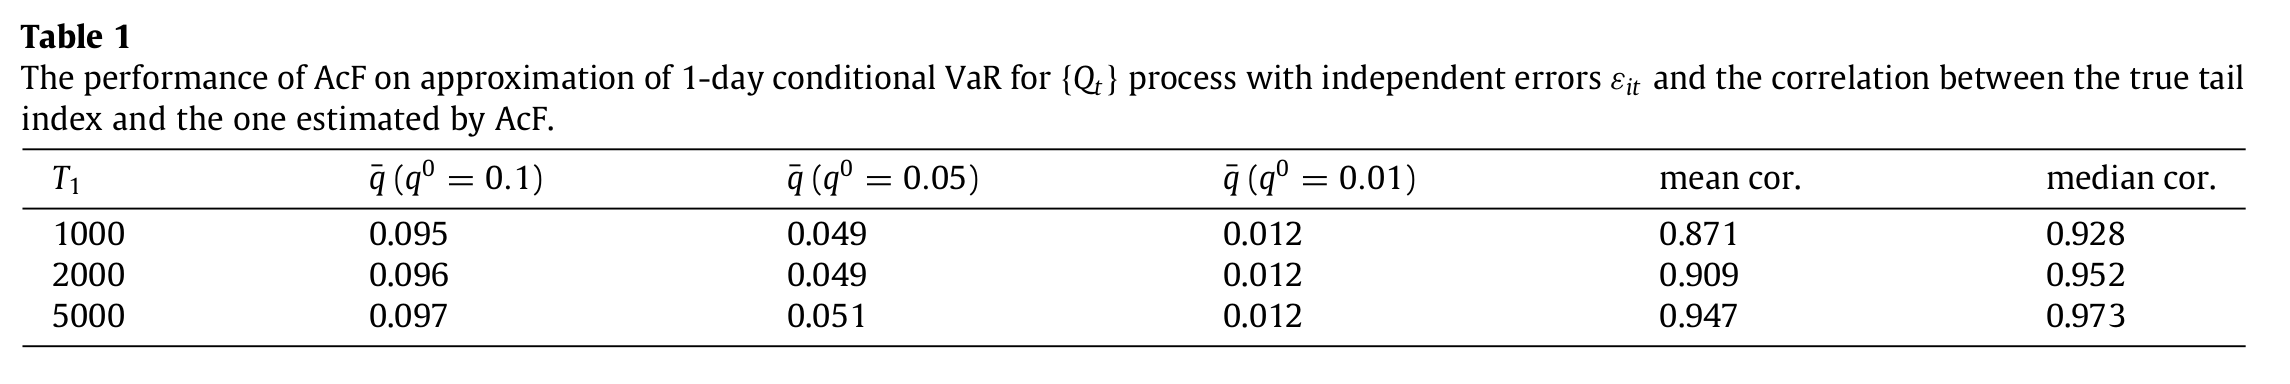
\includegraphics[width=01\textwidth]{table1.png}   
    \end{figure}
\end{frame}





\begin{frame}
    \frametitle{Performance of the MLE}
 To study the finite sample performance of the MLE, simulate the data from an AcF with the following parameters $(\beta_0,\beta_1,\beta_2,\beta_3,\gamma_0,\gamma_1,\gamma_2,\gamma_3,\mu)=(-0.050,0.96,-0.051,6.68,-0.068,0.89,0.33,5.33,-0.069)$

\end{frame}

\begin{frame}
    \frametitle{Simulation Result}
\begin{figure}
    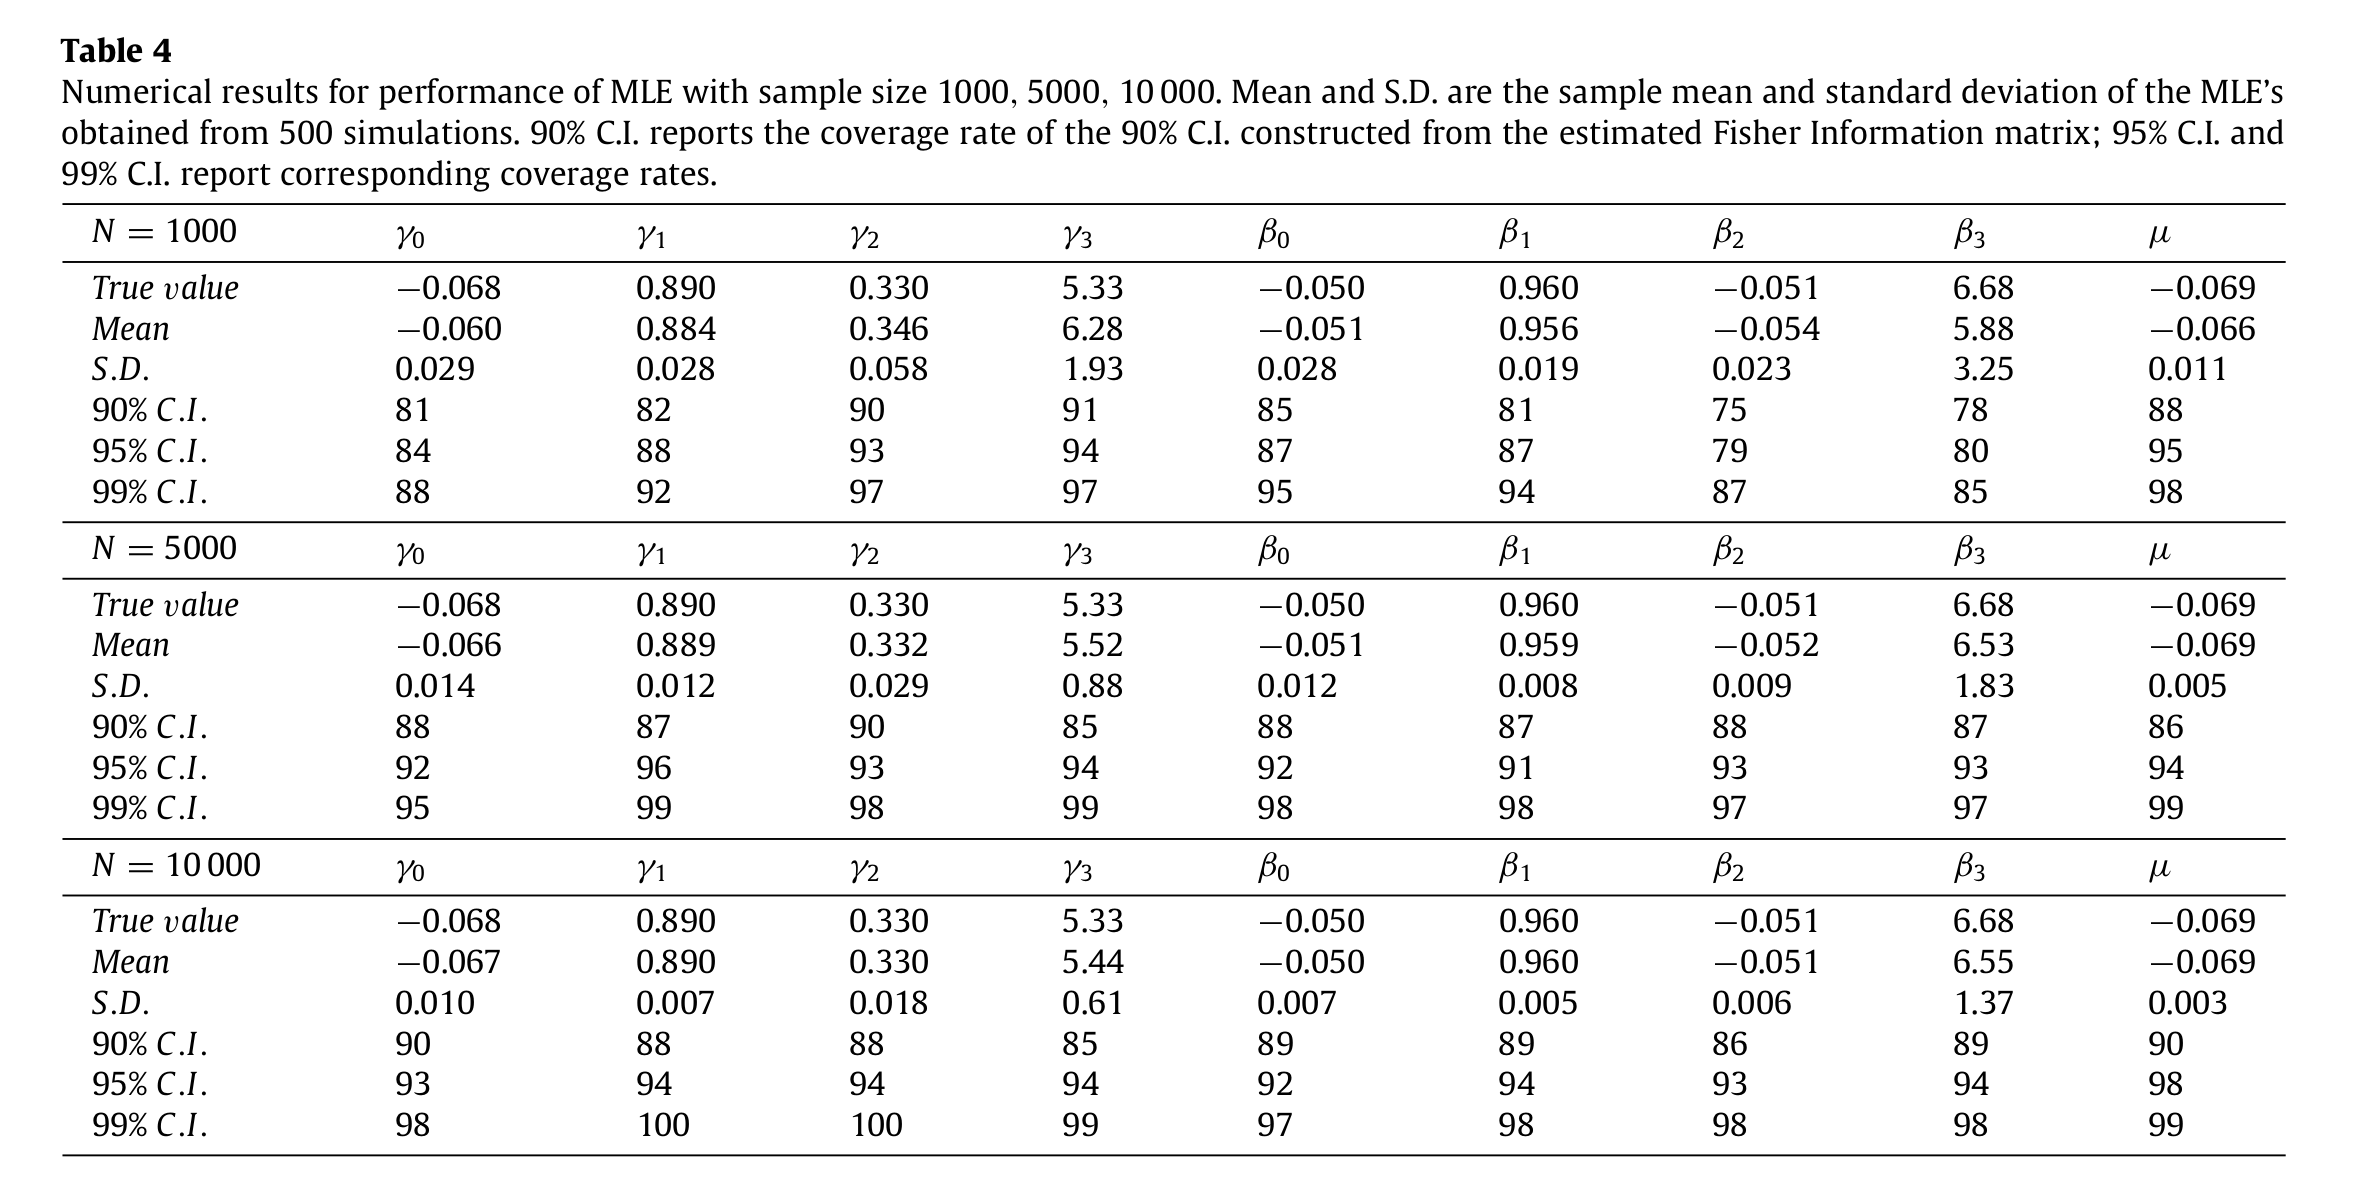
\includegraphics[width=1\textwidth]{table4.png}
\end{figure}
    

\end{frame}


\section{Real Data Applications}



\begin{frame}
    \frametitle{Cross-sectional maxima of the negative daily log-returns of stocks}

    \begin{figure}
        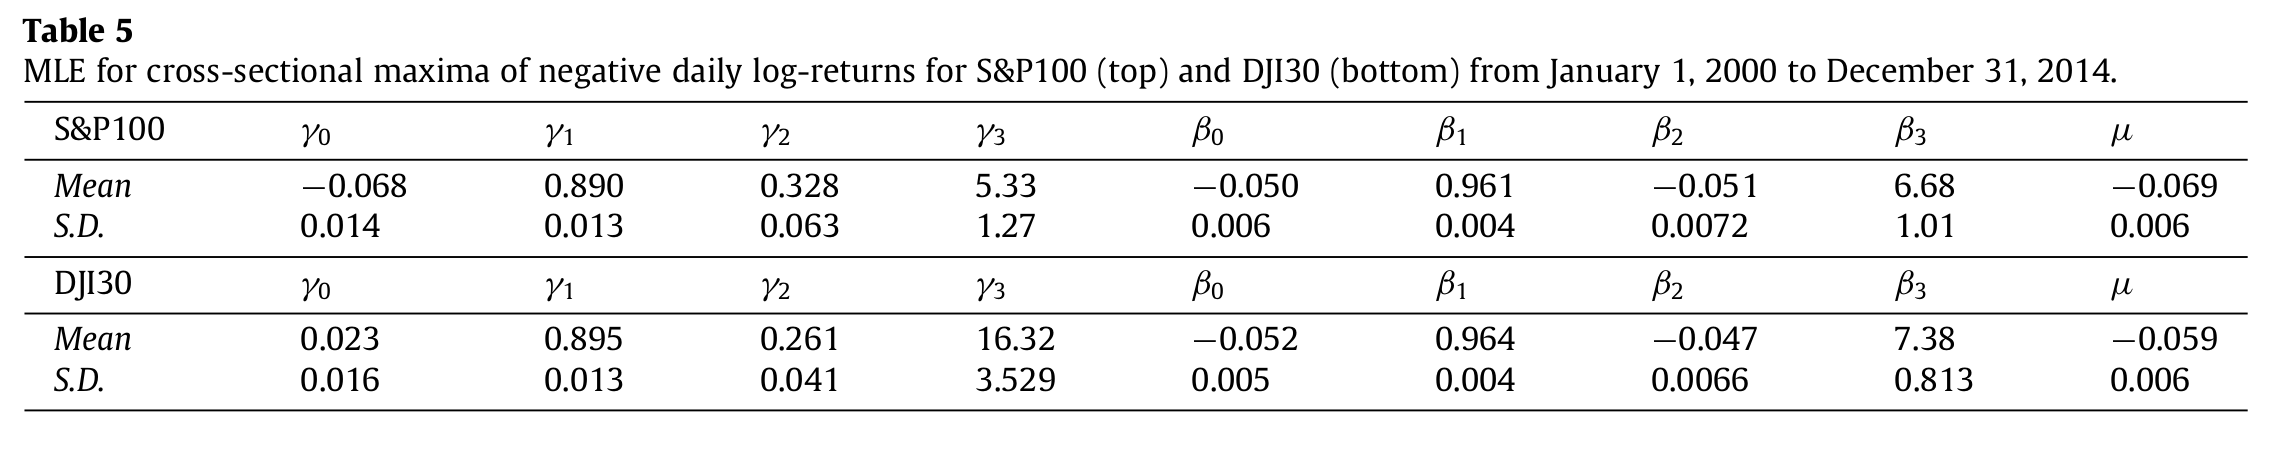
\includegraphics[width=1\textwidth]{table5.png}
    \end{figure}

\end{frame}

\begin{frame}
    \frametitle{Cross-sectional maxima of the negative daily log-returns of stocks}

    \begin{figure}
        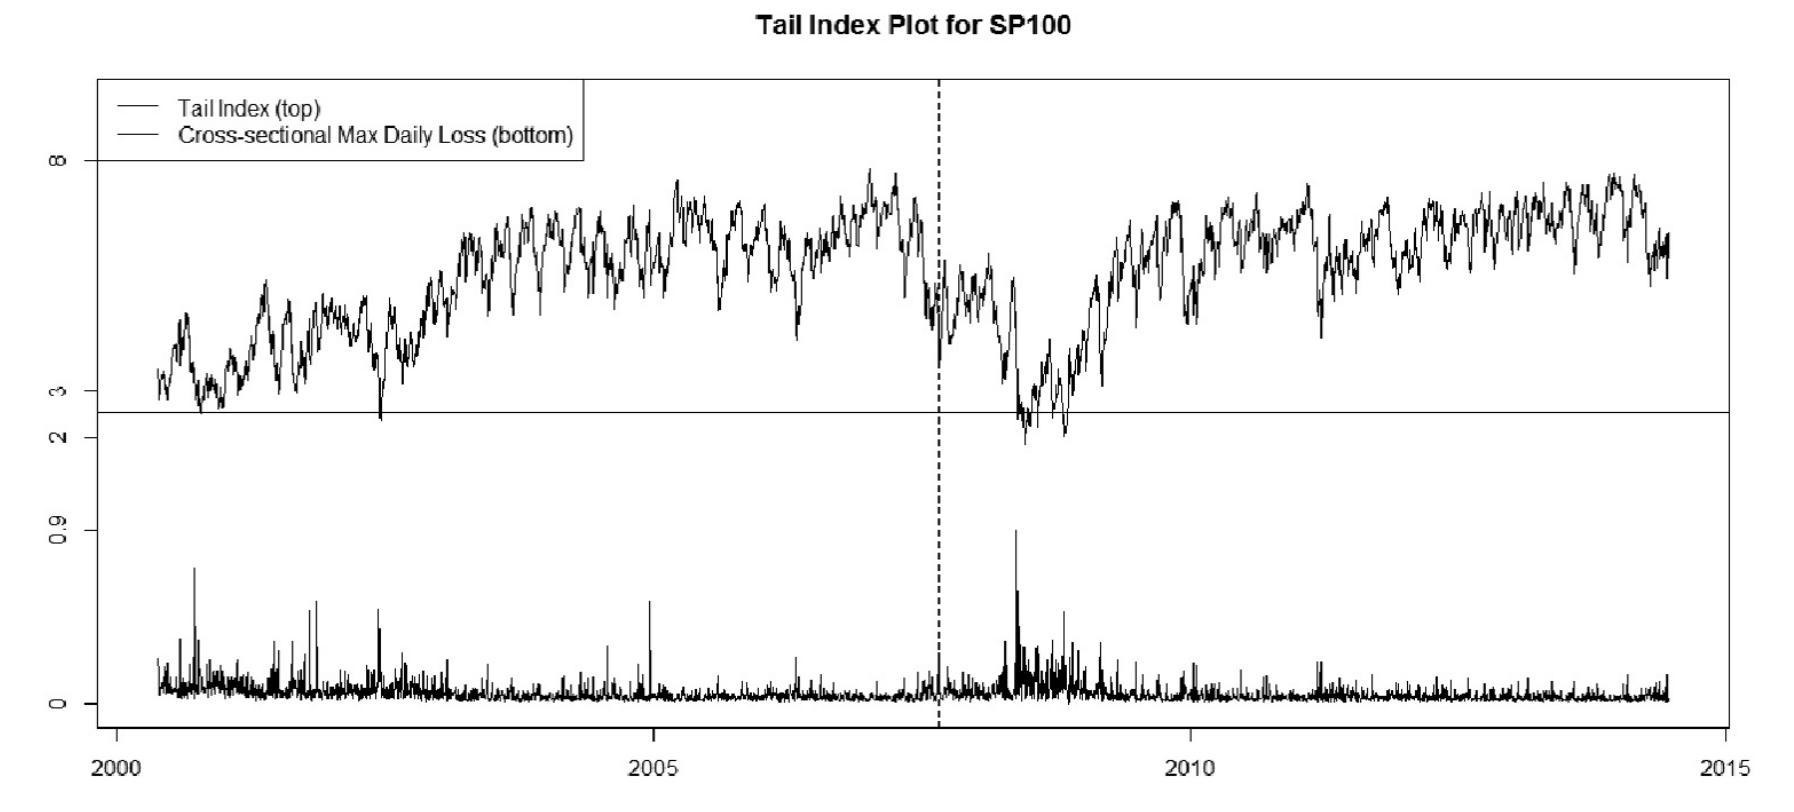
\includegraphics[width=1\textwidth]{fig3.png}
    \end{figure}

\end{frame}



\begin{frame}
    \frametitle{Intra-day maxima of 3-minute negative log-returns for USD/JPY foreign exchange rate}

    \begin{figure}
        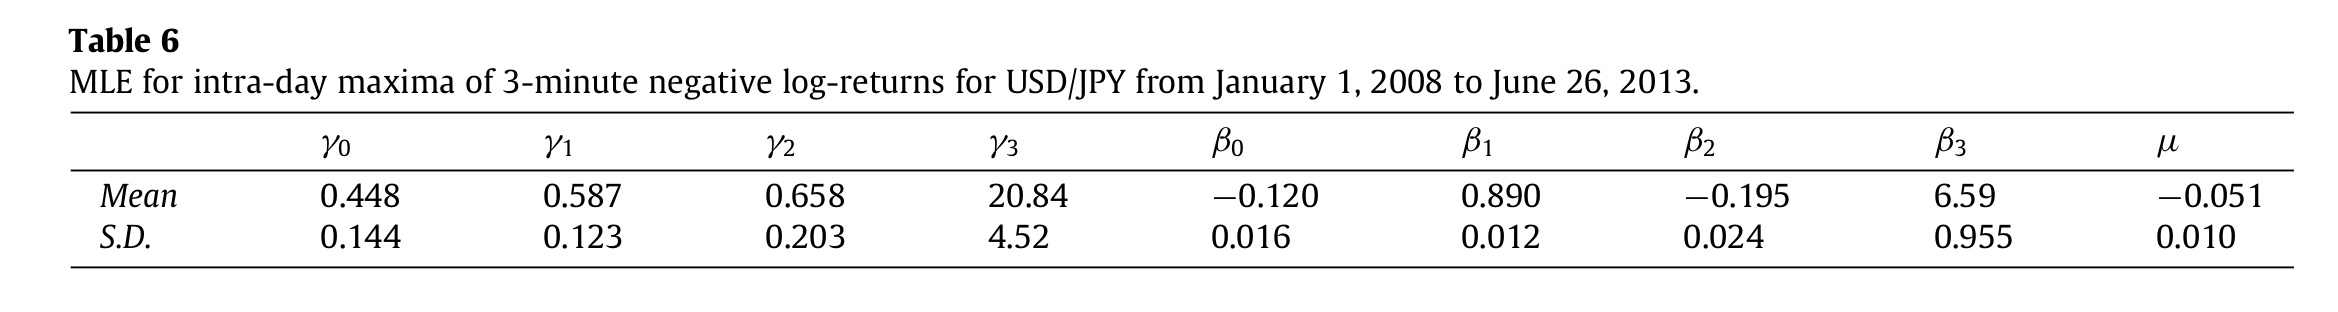
\includegraphics[width=1\textwidth]{table6.png}
    \end{figure}
\end{frame}


\begin{frame}
    \frametitle{Intra-day maxima of 3-minute negative log-returns for USD/JPY foreign exchange rate}

    \begin{figure}
        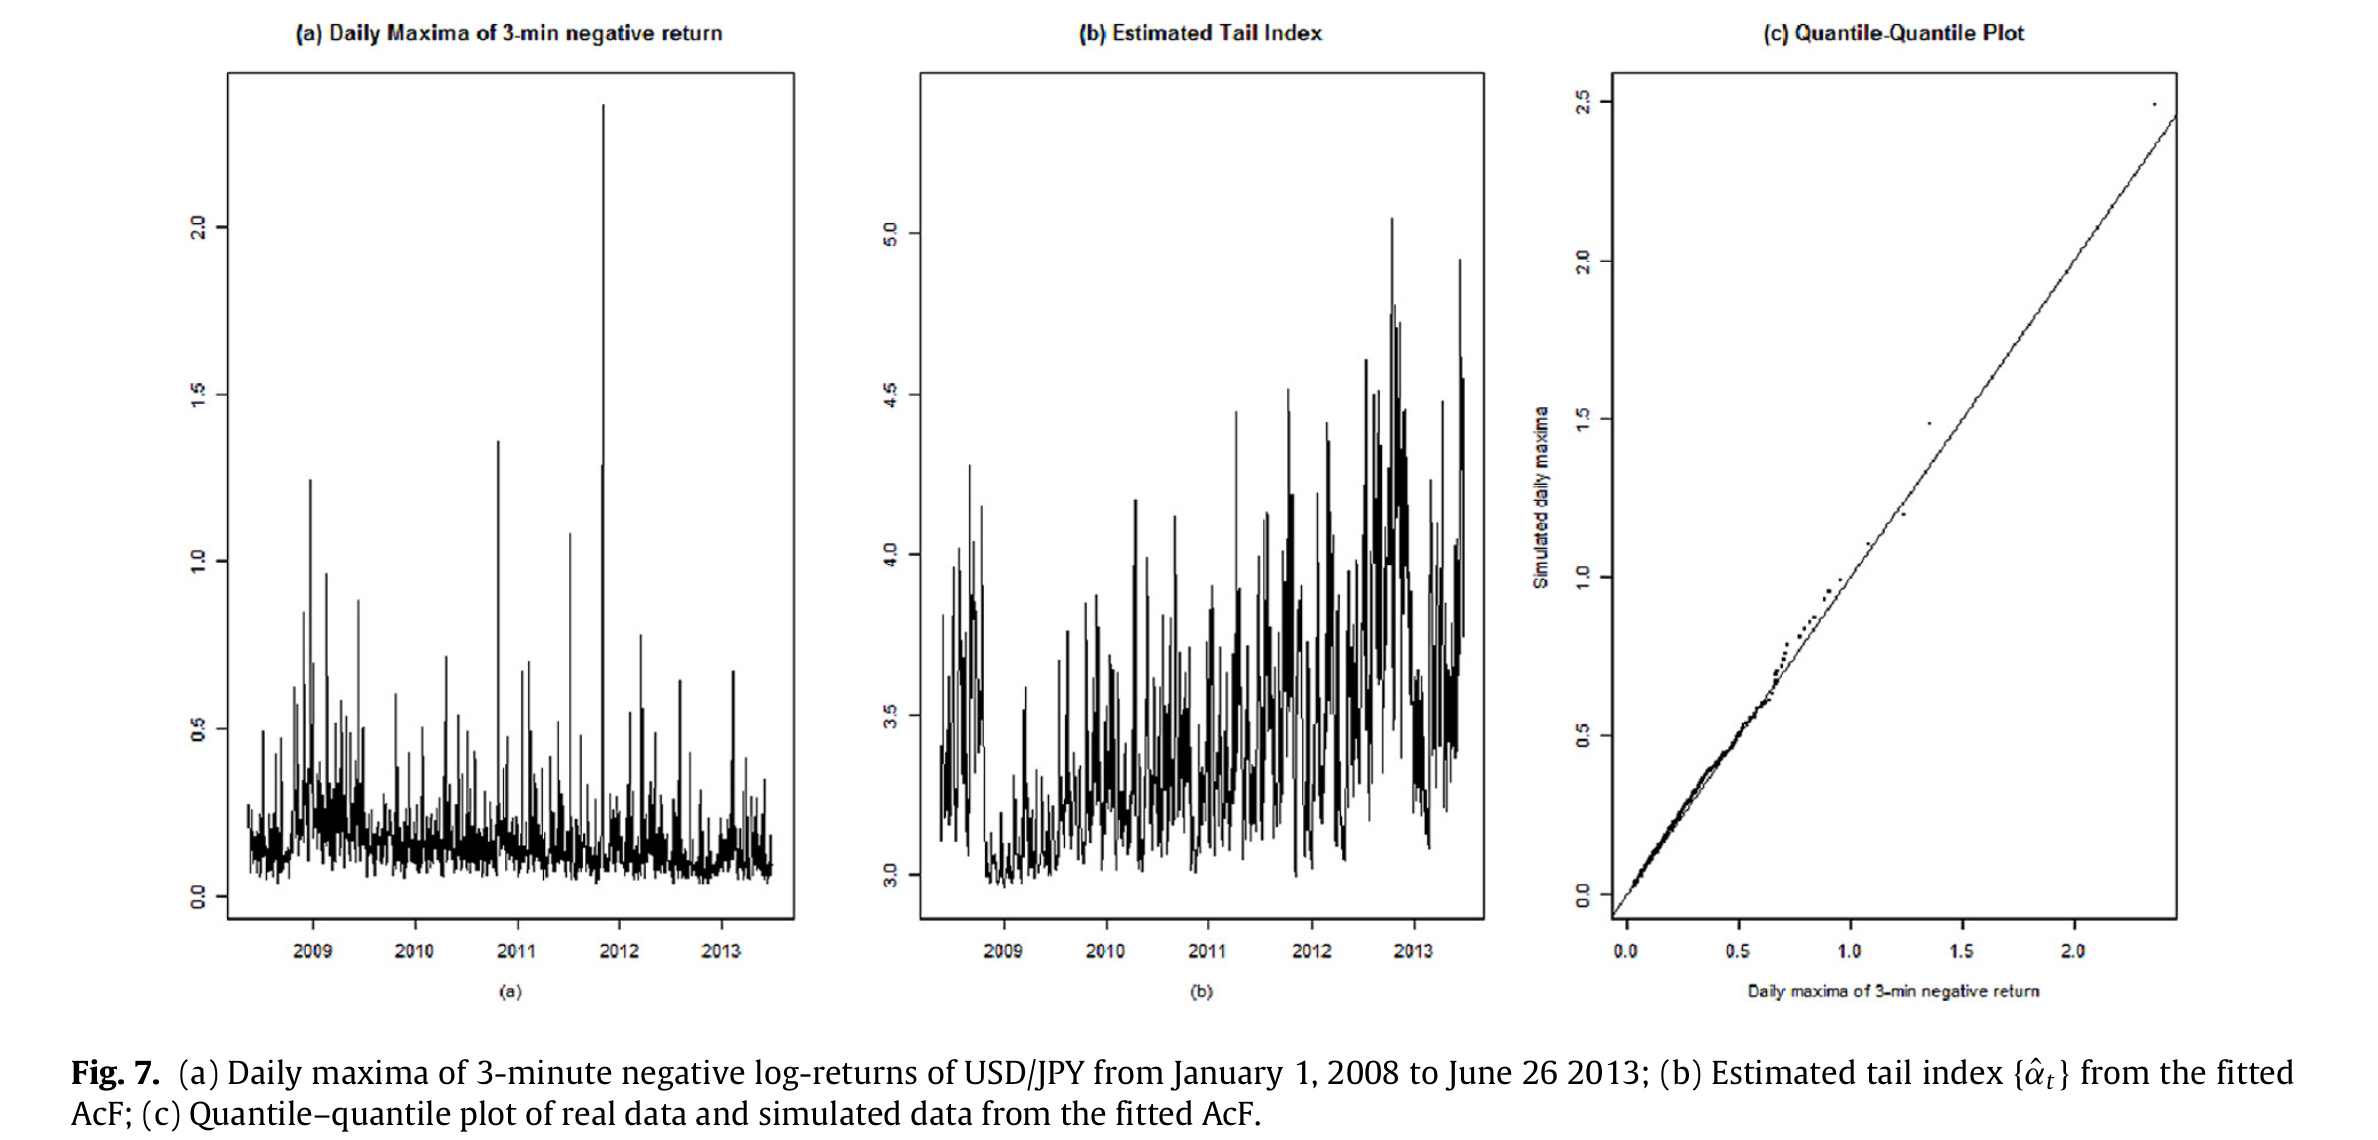
\includegraphics[width=1\textwidth]{fig7.png}
    \end{figure}
\end{frame}
\end{document}